\documentclass[aspectratio=169,11pt]{beamer}
\usepackage[T1]{fontenc}
\usepackage{lmodern,amsmath,amssymb,booktabs,array,multicol}
\usepackage{tikz,pgfplots}
\pgfplotsset{compat=1.18}
\usetheme{default}
\definecolor{navy}{HTML}{000000}
\definecolor{teal}{HTML}{000000}
\definecolor{pale}{HTML}{FFFFFF}
\definecolor{orange}{HTML}{000000}
\setbeamercolor{normal text}{fg=black,bg=white}
\setbeamercolor{structure}{fg=black}
\setbeamercolor{frametitle}{fg=black,bg=white}
\setbeamercolor{title}{fg=black}
\setbeamercolor{subtitle}{fg=black}
\setbeamercolor{block title}{fg=black,bg=white}
\setbeamercolor{block body}{fg=black,bg=white}
\setbeamertemplate{navigation symbols}{}
\setbeamertemplate{footline}{\leavevmode\hbox{\begin{beamercolorbox}[wd=.82\paperwidth,ht=2.5ex,dp=1ex,leftskip=1em]{author in head/foot}\color{navy}\insertshorttitle\end{beamercolorbox}\begin{beamercolorbox}[wd=.18\paperwidth,ht=2.5ex,dp=1ex,center]{date in head/foot}\color{navy}\insertframenumber/\inserttotalframenumber\end{beamercolorbox}}}
\setbeamertemplate{frametitle}{\vspace{0.35em}\insertframetitle\par\vspace{-0.35em}\rule{\textwidth}{0.35pt}}
\setbeamertemplate{blocks}[default]
\setbeamertemplate{itemize item}{\color{black}$\blacktriangleright$}
\newcommand{\key}[1]{\textcolor{black}{\textbf{#1}}}
\newcommand{\source}[1]{\vfill{\tiny\color{gray}Source: #1}}

\title[]{Descriptive Statistics\\From Data Summaries to Model Estimation}
\subtitle{}
\author{Austin Sabu}
\institute{24-502-0101: Mathematics for Computing}
\date{}

\begin{document}
\begin{frame}[plain]
\begin{tikzpicture}[remember picture,overlay]
\node[align=center,text width=.82\paperwidth] at ([yshift=.45cm]current page.center) {\fontsize{26}{31}\selectfont\textbf{Descriptive Statistics}};
\node[anchor=south east,align=right] at ([xshift=-.75cm,yshift=.65cm]current page.south east) {\large Austin Sabu\\[0.2em]\normalsize MTech CSE(AIDS)};
\end{tikzpicture}
\end{frame}

\begin{frame}{What this presentation covers}
\begin{enumerate}
  \item Histograms, mean, variance and order statistics
  \item Covariance and the sample covariance matrix
  \item Frequency statistics and sampling
  \item Mean square error, consistency and confidence intervals
  \item Parametric and non-parametric model estimation
\end{enumerate}
\begin{block}{Learning goal}
Move from describing a sample to judging and communicating how well it estimates an unknown population.
\end{block}
\end{frame}

\begin{frame}{Descriptive statistics turns data into information}
\begin{columns}[T]
\column{0.52\textwidth}
\key{Population} is the complete group of interest. A numerical feature of it is a \key{parameter}, such as $\mu$ or $\sigma^2$.

\medskip
\key{Sample} is the observed subset. A number computed from it is a \key{statistic}, such as $\bar{x}$ or $s^2$.
\column{0.43\textwidth}
\begin{block}{Two descriptive tasks}
\begin{itemize}
  \item Visualize the pattern
  \item Summarize centre, spread and association
\end{itemize}
\end{block}
\end{columns}
\medskip
Descriptive statistics describes the observed data; inferential statistics later uses the sample to learn about the population.
\end{frame}

\begin{frame}{A histogram shows the distribution of numerical data}
For class intervals $I_1,\ldots,I_k$, the frequency of class $j$ is
\[
f_j=\#\{x_i:x_i\in I_j\}, \qquad \sum_{j=1}^{k}f_j=n.
\]
\begin{center}
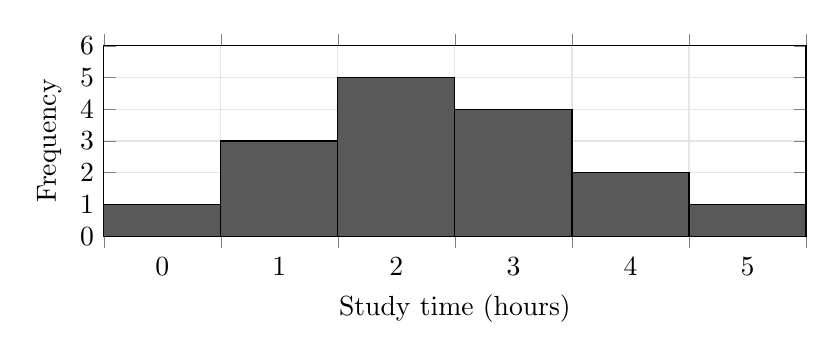
\begin{tikzpicture}
\begin{axis}[ybar interval,width=10.5cm,height=4.0cm,xlabel={Study time (hours)},ylabel={Frequency},xmin=0,xmax=6,ymin=0,ymax=6,xtick={0,1,2,3,4,5,6},ytick={0,1,...,6},grid=major,grid style={gray!20}]
\addplot[fill=teal!65,draw=navy] coordinates {(0,1)(1,3)(2,5)(3,4)(4,2)(5,1)(6,0)};
\end{axis}
\end{tikzpicture}
\end{center}
Touching bars emphasize that the variable is quantitative and intervals are continuous.
\end{frame}

\begin{frame}{Building a histogram is a sequence of choices}
\begin{enumerate}
  \item Find the range: $R=x_{\max}-x_{\min}$.
  \item Choose a reasonable number of classes $k$.
  \item Select width $h\approx R/k$ and convenient boundaries.
  \item Count observations in each interval.
  \item Draw adjacent bars; label axes and units.
\end{enumerate}
\begin{block}{Important caution}
Different bin widths can reveal or hide features. Very few bins oversmooth; too many bins create noise. Report the interval convention, such as $[a,b)$.
\end{block}
\end{frame}

\begin{frame}{Read shape, centre, spread and unusual values}
\begin{columns}[T]
\column{0.50\textwidth}
From a histogram ask:
\begin{itemize}
  \item Is it symmetric or skewed?
  \item Is it unimodal or multimodal?
  \item Where is its typical centre?
  \item How wide is the distribution?
  \item Are there gaps or outliers?
\end{itemize}
\column{0.45\textwidth}
\begin{block}{Histogram limitations}
Exact observations and their original order are lost. Histograms describe one numerical variable; they do not by themselves explain cause.
\end{block}
\end{columns}
\end{frame}

\begin{frame}{The sample mean is the balance point}
For observations $x_1,\ldots,x_n$,
\[
\boxed{\bar{x}=\frac{1}{n}\sum_{i=1}^{n}x_i}
\]
Example: for $2,4,4,5,5$, $\bar{x}=20/5=4$.

\medskip
\begin{block}{Key properties}
\begin{itemize}
  \item $\sum_{i=1}^{n}(x_i-\bar{x})=0$.
  \item It uses every observation.
  \item It is sensitive to extreme values.
  \item Under $y_i=a+bx_i$, $\bar{y}=a+b\bar{x}$.
\end{itemize}
\end{block}
\end{frame}

\begin{frame}{Variance measures squared distance from the mean}
The sample variance and sample standard deviation are
\[
\boxed{s^2=\frac{1}{n-1}\sum_{i=1}^{n}(x_i-\bar{x})^2},\qquad \boxed{s=\sqrt{s^2}}.
\]
\begin{itemize}
  \item $s^2\ge 0$ and equals zero only when all values are identical.
  \item Variance has squared units; standard deviation has the original units.
  \item The denominator $n-1$ gives the usual unbiased estimator of population variance for an i.i.d. sample.
\end{itemize}
\textbf{Computational identity:}
\[
s^2=\frac{\sum x_i^2-n\bar{x}^{2}}{n-1}.
\]
\end{frame}

\begin{frame}{Worked example: mean and variance}
Data: $2,4,4,5,5$. We found $\bar{x}=4$.
\begin{center}
\begin{tabular}{c@{\qquad}c@{\qquad}c}
\toprule
$x_i$ & $x_i-\bar{x}$ & $(x_i-\bar{x})^2$\\
\midrule
2 & $-2$ & 4\\
4 & 0 & 0\\
4 & 0 & 0\\
5 & 1 & 1\\
5 & 1 & 1\\
\midrule
Total & 0 & 6\\
\bottomrule
\end{tabular}
\end{center}
\[
s^2=\frac{6}{5-1}=1.5,\qquad s=\sqrt{1.5}\approx1.225.
\]
Interpretation: observations typically differ from the mean by roughly $1.225$ units.
\end{frame}

\begin{frame}{Order statistics describe position after sorting}
Sort a sample into
\[
X_{(1)}\le X_{(2)}\le\cdots\le X_{(n)}.
\]
Here $X_{(r)}$ is the $r$th \key{order statistic}; parentheses indicate rank, not the original observation number.
\begin{itemize}
  \item Minimum: $X_{(1)}$
  \item Maximum: $X_{(n)}$
  \item Range: $X_{(n)}-X_{(1)}$
  \item Median: middle order statistic (or mean of two middle values)
  \item Quartiles and percentiles: selected ranked positions
\end{itemize}
\end{frame}

\begin{frame}{Order statistics support robust summaries}
For $3,5,6,8,11,13,17$:
\[
X_{(1)}=3,\quad X_{(4)}=8,\quad X_{(7)}=17.
\]
Thus the median is 8 and the range is $17-3=14$.

\medskip
\begin{block}{Why ranking matters}
The median and interquartile range depend on order rather than the numerical size of every deviation. They are therefore less affected by a single extreme value than the mean and variance.
\end{block}
In probability theory, order statistics themselves are random variables because a different random sample gives different ranked values.
\end{frame}

\begin{frame}{Covariance measures joint linear movement}
For paired observations $(x_i,y_i)$,
\[
\boxed{s_{xy}=\frac{1}{n-1}\sum_{i=1}^{n}(x_i-\bar{x})(y_i-\bar{y})}
\]
\begin{columns}[T]
\column{0.31\textwidth}
\key{$s_{xy}>0$}\\Large $x$ and $y$ tend to rise together.
\column{0.31\textwidth}
\key{$s_{xy}<0$}\\Large One tends to fall as the other rises.
\column{0.31\textwidth}
\key{$s_{xy}\approx0$}\\Large Little linear co-movement.
\end{columns}
\medskip
Zero covariance does not generally imply independence, and covariance does not prove causation.
\end{frame}

\begin{frame}{Worked example: sample covariance}
Let $x=(1,2,3)$ and $y=(2,4,5)$. Then $\bar{x}=2$ and $\bar{y}=11/3$.
\begin{center}
\begin{tabular}{ccccc}
\toprule
$i$ & $x_i$ & $y_i$ & $x_i-\bar{x}$ & $(x_i-\bar{x})(y_i-\bar{y})$\\
\midrule
1 & 1 & 2 & $-1$ & $5/3$\\
2 & 2 & 4 & 0 & 0\\
3 & 3 & 5 & 1 & $4/3$\\
\bottomrule
\end{tabular}
\end{center}
\[
s_{xy}=\frac{(5/3)+0+(4/3)}{3-1}=\frac{3}{2}=1.5.
\]
The positive sign matches the visible tendency: larger $x$ is paired with larger $y$.
\end{frame}

\begin{frame}{Covariance depends on measurement scale}
If $u=a+bx$ and $v=c+dy$, then
\[
s_{uv}=bd\,s_{xy}.
\]
So converting metres to centimetres multiplies covariance by 100 if only one variable is converted, or by $10{,}000$ if both are converted.

\begin{block}{Standardized alternative}
Pearson's sample correlation removes units:
\[
r=\frac{s_{xy}}{s_xs_y},\qquad -1\le r\le1.
\]
Correlation is included here only to interpret covariance; the required endpoint of this presentation is sample covariance.
\end{block}
\end{frame}

\begin{frame}{One dataset, five complementary views}
\begin{center}
\begin{tabular}{>{\bfseries}l p{8.3cm}}
\toprule
Tool & Question answered\\
\midrule
Histogram & What is the overall shape of one variable?\\
Sample mean & Where is the arithmetic centre?\\
Sample variance & How dispersed are observations around the mean?\\
Order statistics & What are the ranked positions and robust summaries?\\
Sample covariance & How do two variables vary together linearly?\\
\bottomrule
\end{tabular}
\end{center}
No single summary is sufficient: good analysis combines a graph, numerical summaries, and context.
\end{frame}

\begin{frame}{A covariance matrix summarizes multivariate spread}
For $p$ measured variables, let $\mathbf{x}_i=(x_{i1},\ldots,x_{ip})^T$ and sample mean vector $\bar{\mathbf{x}}$. The sample covariance matrix is
\[
\boxed{\mathbf{S}=\frac{1}{n-1}\sum_{i=1}^{n}(\mathbf{x}_i-\bar{\mathbf{x}})(\mathbf{x}_i-\bar{\mathbf{x}})^T}.
\]
Its $(j,k)$ entry is $s_{jk}$, the covariance between variables $j$ and $k$.
\[
\mathbf{S}=\begin{pmatrix}
s_1^2&s_{12}&\cdots&s_{1p}\\
s_{21}&s_2^2&\cdots&s_{2p}\\
\vdots&\vdots&\ddots&\vdots\\
s_{p1}&s_{p2}&\cdots&s_p^2
\end{pmatrix}.
\]
\end{frame}

\begin{frame}{The covariance matrix has useful structure}
\begin{itemize}
  \item \key{Symmetric:} $s_{jk}=s_{kj}$, so $\mathbf{S}=\mathbf{S}^T$.
  \item \key{Diagonal:} $s_{jj}=s_j^2$, the sample variance of variable $j$.
  \item \key{Positive semidefinite:} for any vector $\mathbf{a}$,
  \[
  \mathbf{a}^T\mathbf{S}\mathbf{a}\ge0.
  \]
  \item \key{Scale-dependent:} changing units changes relevant rows and columns.
\end{itemize}
\begin{block}{Why it matters in computing}
Covariance matrices appear in PCA, Gaussian models, anomaly detection, Kalman filtering and portfolio/risk calculations.
\end{block}
\end{frame}

\begin{frame}{Worked covariance matrix}
Suppose two variables have $s_x^2=4$, $s_y^2=9$ and $s_{xy}=3$. Then
\[
\mathbf{S}=\begin{pmatrix}4&3\\3&9\end{pmatrix}.
\]
The corresponding correlation is
\[
r_{xy}=\frac{3}{\sqrt{4}\sqrt{9}}=\frac12.
\]
\begin{itemize}
  \item Diagonal entries report individual spreads.
  \item Off-diagonal entries report joint movement.
  \item Symmetry avoids storing duplicate information.
\end{itemize}
\end{frame}

\begin{frame}{Frequency statistics count how often outcomes occur}
For a value or class $A_j$:
\[
f_j=\#\{i:x_i\in A_j\},\qquad r_j=\frac{f_j}{n},\qquad c_j=\sum_{\ell\le j}f_\ell.
\]
\begin{center}
\begin{tabular}{lccc}
\toprule
Score interval & Frequency $f_j$ & Relative frequency $r_j$ & Cumulative $c_j$\\
\midrule
0--9 & 2 & 0.10 & 2\\
10--19 & 6 & 0.30 & 8\\
20--29 & 8 & 0.40 & 16\\
30--39 & 4 & 0.20 & 20\\
\bottomrule
\end{tabular}
\end{center}
Relative frequencies sum to 1; cumulative frequency never decreases.
\end{frame}

\begin{frame}{A sample must represent the target population}
\begin{columns}[T]
\column{0.48\textwidth}
\key{Probability sampling}
\begin{itemize}
  \item Simple random
  \item Systematic
  \item Stratified
  \item Cluster
\end{itemize}
\column{0.47\textwidth}
\key{Non-probability sampling}
\begin{itemize}
  \item Convenience
  \item Voluntary response
  \item Judgment/purposive
\end{itemize}
\end{columns}
\begin{block}{Sampling error versus bias}
Sampling error is random sample-to-sample variation. Bias is systematic distortion caused by the design, nonresponse, measurement, or coverage. A large biased sample can still be misleading.
\end{block}
\end{frame}

\begin{frame}{A statistic has its own sampling distribution}
Imagine drawing every possible random sample of size $n$ and calculating $T$ each time. The distribution of those values is the \key{sampling distribution} of $T$.
\begin{block}{For the sample mean of i.i.d. observations}
\[
E(\bar{X})=\mu,\qquad \operatorname{Var}(\bar{X})=\frac{\sigma^2}{n},\qquad \operatorname{SE}(\bar{X})=\frac{\sigma}{\sqrt n}.
\]
\end{block}
Larger samples reduce standard error at the rate $1/\sqrt n$: quadrupling $n$ halves the standard error.
\end{frame}

\begin{frame}{Mean square error combines bias and variability}
For estimator $\hat\theta$ of parameter $\theta$,
\[
\boxed{\operatorname{MSE}(\hat\theta)=E[(\hat\theta-\theta)^2]}
\]
and
\[
\boxed{\operatorname{MSE}(\hat\theta)=\operatorname{Var}(\hat\theta)+\operatorname{Bias}(\hat\theta)^2},
\quad \operatorname{Bias}(\hat\theta)=E(\hat\theta)-\theta.
\]
\begin{block}{Interpretation}
MSE penalizes large errors quadratically. A slightly biased estimator can have lower MSE if it greatly reduces variance; this is the bias--variance trade-off.
\end{block}
\end{frame}

\begin{frame}{Deriving the bias--variance decomposition}
Write $b=E(\hat\theta)-\theta$ and add/subtract $E(\hat\theta)$:
\begin{align*}
E[(\hat\theta-\theta)^2]
&=E[(\hat\theta-E\hat\theta+b)^2]\\
&=E[(\hat\theta-E\hat\theta)^2]
+2bE[\hat\theta-E\hat\theta]+b^2\\
&=\operatorname{Var}(\hat\theta)+b^2.
\end{align*}
The cross-term vanishes because $E[\hat\theta-E(\hat\theta)]=0$.

\medskip
If $\hat\theta$ is unbiased, then $\operatorname{MSE}(\hat\theta)=\operatorname{Var}(\hat\theta)$.
\end{frame}

\begin{frame}{Consistency means error vanishes with more data}
An estimator sequence $\hat\theta_n$ is \key{consistent} for $\theta$ if
\[
\hat\theta_n\xrightarrow{P}\theta,
\]
meaning that for every $\varepsilon>0$,
\[
P(|\hat\theta_n-\theta|>\varepsilon)\longrightarrow0.
\]
\begin{block}{Useful sufficient condition}
If $\operatorname{MSE}(\hat\theta_n)\to0$, then $\hat\theta_n$ is consistent, by Markov/Chebyshev inequality.
\end{block}
For i.i.d. observations with finite variance, $\bar X_n$ is consistent because its bias is 0 and its variance is $\sigma^2/n\to0$.
\end{frame}

\begin{frame}{Unbiased and consistent are different ideas}
\begin{center}
\begin{tabular}{>{\bfseries}p{3cm}p{4.1cm}p{4.1cm}}
\toprule
Property & Main question & Mathematical idea\\
\midrule
Unbiasedness & Correct on average at a fixed $n$? & $E(\hat\theta_n)=\theta$\\
Consistency & Converges as $n\to\infty$? & $\hat\theta_n\xrightarrow{P}\theta$\\
Efficiency & How variable is it? & Compare variances/MSE\\
\bottomrule
\end{tabular}
\end{center}
An estimator may be biased for every finite $n$ yet consistent if its bias and variance both approach zero.
\end{frame}

\begin{frame}{A confidence interval quantifies estimation uncertainty}
A two-sided $(1-\alpha)100\%$ confidence interval has the form
\[
\boxed{\text{point estimate}\ \pm\ \text{critical value}\times\text{standard error}}.
\]
For a population mean with known $\sigma$,
\[
\bar{x}\pm z_{\alpha/2}\frac{\sigma}{\sqrt n}.
\]
For unknown $\sigma$ and an approximately normal population,
\[
\bar{x}\pm t_{\alpha/2,n-1}\frac{s}{\sqrt n}.
\]
\end{frame}

\begin{frame}{Worked 95\% confidence interval}
A sample has $n=25$, $\bar{x}=72$ and $s=10$. With $24$ degrees of freedom, $t_{0.025,24}\approx2.064$.
\[
\operatorname{SE}(\bar{x})=\frac{10}{\sqrt{25}}=2,
\]
\[
72\pm2.064(2)=72\pm4.128=(67.872,76.128).
\]
\begin{block}{Correct interpretation}
If this sampling procedure were repeated many times, about 95\% of the intervals constructed this way would contain the fixed population mean $\mu$.
\end{block}
It is not correct to say there is a 95\% probability that this already-computed interval contains a fixed $\mu$ under the frequentist interpretation.
\end{frame}

\begin{frame}{Confidence width reflects a three-way trade-off}
For $\bar{x}\pm z_{\alpha/2}\sigma/\sqrt n$, the margin of error is
\[
E=z_{\alpha/2}\frac{\sigma}{\sqrt n}.
\]
\begin{itemize}
  \item Higher confidence $\Rightarrow$ larger critical value $\Rightarrow$ wider interval.
  \item More variability $\Rightarrow$ larger standard error $\Rightarrow$ wider interval.
  \item Larger $n$ $\Rightarrow$ smaller standard error $\Rightarrow$ narrower interval.
\end{itemize}
To target a margin $E$ when $\sigma$ is known,
\[
n\ge\left(\frac{z_{\alpha/2}\sigma}{E}\right)^2,
\]
rounded upward.
\end{frame}

\begin{frame}{Parametric estimation assumes a finite-dimensional model}
Choose a distribution family $f(x;\theta)$ described by a fixed number of parameters. Examples:
\begin{itemize}
  \item Bernoulli$(p)$: estimate $p$.
  \item Poisson$(\lambda)$: estimate $\lambda$.
  \item Normal$(\mu,\sigma^2)$: estimate $\mu$ and $\sigma^2$.
\end{itemize}
\begin{block}{Common methods}
\key{Method of moments} matches theoretical moments to sample moments. \key{Maximum likelihood} chooses the parameter that makes the observed data most plausible.
\end{block}
Advantages include compact models and efficient inference when assumptions are suitable; misspecification can create bias.
\end{frame}

\begin{frame}{Maximum likelihood example: Bernoulli data}
For independent $x_i\in\{0,1\}$ from Bernoulli$(p)$,
\[
L(p)=\prod_{i=1}^n p^{x_i}(1-p)^{1-x_i}
=p^{\sum x_i}(1-p)^{n-\sum x_i}.
\]
The log-likelihood is
\[
\ell(p)=\Big(\sum x_i\Big)\log p+\Big(n-\sum x_i\Big)\log(1-p).
\]
Setting $\ell'(p)=0$ gives
\[
\boxed{\hat p_{\mathrm{MLE}}=\frac{1}{n}\sum_{i=1}^n x_i=\bar{x}.}
\]
Thus the observed success proportion estimates the population success probability.
\end{frame}

\begin{frame}{Non-parametric estimation lets shape emerge from data}
Non-parametric methods do not restrict the population to one fixed finite-parameter distributional family.
\begin{itemize}
  \item Empirical CDF: $\hat F_n(x)=n^{-1}\sum_{i=1}^{n}\mathbf{1}(X_i\le x)$.
  \item Histogram density estimate: piecewise constant over bins.
  \item Kernel density estimate:
  \[
  \hat f_h(x)=\frac{1}{nh}\sum_{i=1}^{n}K\!\left(\frac{x-X_i}{h}\right).
  \]
\end{itemize}
Flexibility reduces model assumptions but typically needs more data and introduces tuning choices such as bin width or bandwidth $h$.
\end{frame}

\begin{frame}{Parametric versus non-parametric estimation}
\begin{center}
\begin{tabular}{>{\bfseries}p{2.8cm}p{4.4cm}p{4.4cm}}
\toprule
Feature & Parametric & Non-parametric\\
\midrule
Assumption & Specified family $f(x;\theta)$ & Few shape restrictions\\
Complexity & Fixed-dimensional parameter & Can grow with sample size\\
Strength & Efficient, interpretable & Flexible, robust to shape\\
Risk & Model misspecification & Higher variance/tuning sensitivity\\
Examples & MLE for Normal/Bernoulli & ECDF, histogram, KDE\\
\bottomrule
\end{tabular}
\end{center}
The choice depends on scientific knowledge, sample size, interpretability and predictive goal.
\end{frame}

\begin{frame}{Module 3 forms one connected workflow}
\begin{enumerate}
  \item \key{Inspect}: histogram and frequency statistics reveal pattern.
  \item \key{Summarize}: mean, variance, order statistics and covariance describe the sample.
  \item \key{Generalize}: sampling distributions connect statistics to parameters.
  \item \key{Evaluate}: bias, MSE and consistency judge estimators.
  \item \key{Communicate}: confidence intervals express uncertainty.
  \item \key{Model}: parametric or non-parametric estimation learns population structure.
\end{enumerate}
\end{frame}




\begin{frame}[plain]
\begin{center}
{\Huge\color{navy}\textbf{Thank You}}\\[1em]
\end{center}
\end{frame}
\end{document}
